% Vorlage für eine Bachelorarbeit
% Siehe auch LaTeX-Kurs von Mathematik-Online
% www.mathematik-online.org/kurse
% Anpassungen für die Fakultät für Mathematik
% am KIT durch Klaus Spitzmüller und Roland Schnaubelt im Dezember 2011

\documentclass[11pt,a4paper,titlepage]{scrartcl}
% scrartcl ist eine abgeleitete Artikel-Klasse im Koma-Skript
% zur Kontrolle des Umbruchs Klassenoption draft verwenden

\usepackage{array}
% die folgenden Packete erlauben den Gebrauch von Umlauten und ß
% in der Latex Datei
\usepackage[utf8]{inputenc}
% \usepackage[latin1]{inputenc} %  Alternativ unter Windows
\usepackage[T1]{fontenc}
\usepackage[ngerman]{babel}
\usepackage[babel,german=quotes]{csquotes}
\usepackage[pdftex]{graphicx}
\usepackage{latexsym}
\usepackage{amsmath,amssymb,amsthm}
\usepackage[style=alphabetic,backend=biber]{biblatex}
\usepackage{pdflscape}
\usepackage{colortbl}
\usepackage{color}
\bibliography{bib/Quellen}

\usepackage[footskip=1.5cm, left=2.5cm, right=2.5cm, top=2.5cm, bottom=3.5cm]{geometry}

% Definieren von versch. Farben für Tabellenzellen
\definecolor{grey}{rgb}{0.85,0.85,0.85}
\definecolor{lightgrey}{rgb}{0.95,0.95,0.95}

% Abstand obere Blattkante zur Kopfzeile ist 2.54cm - 15mm
\setlength{\topmargin}{-15mm}
\usepackage[onehalfspacing]{setspace}

% Umgebungen für Definitionen, Sätze, usw.
% Es werden Sätze, Definitionen etc innerhalb einer Section mit
% 1.1, 1.2 etc durchnummeriert, ebenso die Gleichungen mit (1.1), (1.2) ..

\newtheorem{Satz}{Satz}[section]
\newtheorem{Definition}[Satz]{Definition}     
\newtheorem{Lemma}[Satz]{Lemma}	
                  
\numberwithin{equation}{section} 

% einige Abkuerzungen
\newcommand{\C}{\mathbb{C}} % komplexe
\newcommand{\K}{\mathbb{K}} % komplexe
\newcommand{\R}{\mathbb{R}} % reelle
\newcommand{\Q}{\mathbb{Q}} % rationale
\newcommand{\Z}{\mathbb{Z}} % ganze
\newcommand{\N}{\mathbb{N}} % natuerliche

\title{Bachelorarbeit}
\author{Andre Weinkötz (14985714)}
\date{15. Februar 2018}


\begin{document}
  % Keine Seitenzahlen im Vorspann
  \pagestyle{empty}

  % Titelblatt der Arbeit
  \begin{titlepage}

\begin{center}
	\includegraphics[scale=0.20]{img/hm-logo.eps}
\end{center}
 \bigskip

 \begin{center} \large 
    
    Bachelorarbeit im Studiengang B.Sc. Wirtschaftsinformatik
    \vspace*{2.5cm}
\end{center}
\begin{center}
	    {\huge Realisierung einer bidirektionalen Chat-Anwendung durch HTML5 WebSockets mit Java und Angular 4 zum Einsatz im seminaristischen Kontext}
	% Echtzeit-Anwendungen im Web durch WebSockets
\end{center}

    
    \vspace*{2.0cm}
 \begin{center}
    Andre Weinkötz \bigskip
    
    

    15. Februar 2018
    \vspace*{2.5cm}
    
    

    Fakultät für Informatik und Mathematik \\
	Hochschule München\bigskip
	
	Betreuer: Prof. Dr. Mandl 
	
	
  \end{center}
\end{titlepage}

\newpage
\section*{Abstract}
\addcontentsline{toc}{section}{Abstract}
Hier steht am Ende was genau eigentlich mit dem Unsinn hier erreicht werden soll.
\newpage
  % Inhaltsverzeichnis
 \tableofcontents

\newpage
%\textbf{ABSTRACT}
%\newpage
  % Ab sofort Seitenzahlen in der Kopfzeile anzeigen
  \pagestyle{headings}

\section{Einleitung}\label{sec:Einleitung}
Die Anforderungen an Webanwendungen haben sich in den vergangenen Jahren stark verändert. Mobile Geräte wie Smartphones oder Tablets ersetzen stationäre Systeme, Webanwendungen sollen zur Kollaboration eingesetzt werden und Buchungssysteme oder Finanzanwendungen verlangen die Bearbeitung tausender Anfragen mit minimaler Verzögerung. Das Hypertext Transfer Protocol (HTTP) bietet hier keine zufriedenstellende Lösung. Um den Anforderungen an moderne Webanwendungen gerecht zu werden, spezifizierten das World Wide Web Consortium (W3C) und die Internet Engineering Taskforce (IETF) das WebSocket-Protokoll mit zugehöriger JavaScript-API. \\

\noindent Die Entwickler des WebSocket Protokolls machten es sich zur Aufgabe, einen Mechanismus zu schaffen, der es browserbasierten Anwendungen ermöglicht bidirektional zu kommunizieren ohne dabei auf mehrere HTTP Verbindungen zu öffnen \autocite{fette_websocket_2011}. Dabei sollte auf zusätzliche Methoden - wie beispielsweise den Einsatz von XMLHttpRequests, iframes oder long polling - verzichtet werden.

\newpage
\section{Das WebSocket Protokoll}\label{sec:WebSocketProtokoll}
Die Arbeit an der Spezifikation des WebSocket Protokolls begann bereits 2009, als es von Google in Zusammenarbeit mit Apple, Microsoft und Mozilla im Rahmen ihrer Kooperation WHATWG\footnote{Web Hypertext Application Technology Working Group unter: www.whatwg.org} der Internet Engineering Task Force (IETF) vorgeschlagen wurde. Bis Mai 2010 wurden noch zahlreiche Verbesserungen hinzugefügt, bis es schließlich in Version 76 \autocite{hickson_websocket_2010} im August 2010 an die BiDirectional or Server-Initiated HTTP (HyBi) Task Force der IETF zur Weiterentwicklung übergeben wurde \autocite{fette_websocket_2010}. Neben vielen anderen Fortschritten wurde das Protkoll um die Möglichkeit erweitert binäre Dateien auszutauschen, sowie Sicherheitslücken geschlossen, die in Verbindung mit Proxy-Servern entstehen konnten. Im Dezember 2010 wurde das WebSocket Protokoll von der IETF zu dem Request for Comment (RFC) 6455 erklärt \autocite{fette_websocket_2011}. Dieser definiert auf über 70 Seiten neben dem Lebenszyklus und den verschiedenen Frames der WebSockets noch zahlreiche weitere technische Details und Defintionen. In diesem Kapitel sollen die wichtigsten Grundlagen der Protokollspezifikation dargelegt werden.
\subsection{WebSocket-Frames}\label{subsec:wsFrames}
Die Spezifikation eines WebSocket-Frames sieht eine Zweiteilung vor, wie sie bei Protokollnachrichten üblicherweise vorgenommen wird. Ein WebSocket-Frame besteht demnach aus einem Header Bereich der Kontrolldaten enthält, sowie dem Payload, welcher die Nutzdaten beinhaltet.\vspace{2mm}
\begin{figure}[ht] \label{fig:wsFrame}
	\begin{center}
		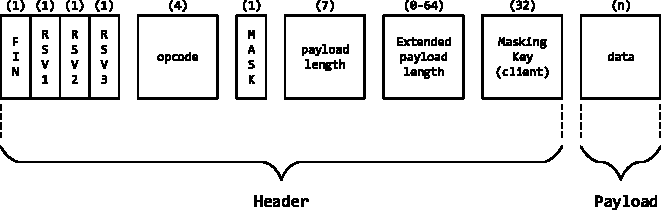
\includegraphics[scale=1.25]{img/frame.pdf}
		\caption{Vereinfachte Darstellung eines WebSocket Frames}
	\end{center}
\end{figure}
Anhand des Aufbaus ist leicht erkennbar, dass die Kommunikation über WebSockets mit deutlich geringeren Paketgrößen arbeiten kann als HTTP. Eine Nachricht mit einfacher Längenangabe, die von Server zu Client geschickt wird, erzeugt durch ihren Header lediglich einen Overhead von zwei Byte. Da WebSocket-Frames auf umgekehrtem Weg zusätzlich noch maskiert werden müssen, entspricht die minimale Länge eines clientseitigen Frames sechs Byte. Im Vergleich dazu beträgt der Overhead bei einer einfachen GET-Anfrage über HTTP/1.1 beim Aufruf des Hosts unter cs.hm.edu 35 Byte. Die Angabe des Hostnamens in HTTP/1.1 ist obligatorisch und trägt maßgeblich zur Größe des HTTP-Frames bei \autocite[128]{leach_hypertext_1999}. 

\subsubsection{Header-Felder}\label{subsubsec:wsHeader}
Im nachfolgenden Abschnitt werden die Felder sowie deren jeweilige Aufgabe detailliert erläutert:

\begin{description}
	\item[FIN (1 Bit)] Das FIN-Flag gibt an, ob es sich bei dem empfangenen Frame um ein Fragment handelt. Kann der Payload nicht auf einmal übertragen werden, so wird die Übertragung über mehrere Frames gesteuert. Das FIN-Flag aller unvollständigen Fragmente weist den Wert 0 auf, wohingegen das finale Fragment mit einer 1 gekennzeichnet ist. Wenn alle Nutzdaten mit einem einzigen Frame übertragen werden können, so trägt dessen FIN-Flag ebenfalls den Wert 1.
	\item[RSV1, RSV2, RSV3 (jeweils 1 Bit)] Diese Flags sind für zukünftige Implementierung reserviert und finden aktuell keine standardisierte Anwendung. Die Ausnahme stellt das RSV1-Bit dar, welches verwendet wird um anzuzeigen, ob eine Nachricht komprimiert wurde oder nicht \autocite{internet_assigned_numbers_authority_websocket_2011}. Daher tragen sie meist den Wert 0. Ist eines dieser Flags gesetzt und die empfangende Stelle hat keine Erweiterung, welches das jeweilige Flag interpretieren kann, so muss die WebSocket-Verbindung geschlossen werden \autocite[27]{fette_websocket_2011}. 
	\item[opcode (4 Bit)] Das opcode-Feld enthält die Angabe wie der Payload zu interpretieren ist. Neben den sogenannten Datenframes bzw. Non-Control-Frames, welche die Art der übertragenen Daten kennzeichnen, sind Control-Frames definiert, die zur Steuerung und Überprüfung der Verbindung verwendet werden. Wird ein unbekannter Opcode empfangen, so wird die WebSocket-Verbindung geschlossen.
	\begin{itemize}
		\item \textbf{0x0} definiert ein Fortsetzungs-Frame
		\item \textbf{0x1} definiert ein Text-Frame
		\item \textbf{0x2} definiert ein Binary-Frame
		\item \textbf{0x3-7} reserviert für weitere Non-Control-Frames
		\item \textbf{0x8} definiert ein Verbindung beenden-Frame
		\item \textbf{0x9} definiert ein Ping-Frame
		\item \textbf{0xA} definiert ein Pong-Frame
		\item \textbf{0xB-F} reserviert für weitere Control-Frames
	\end{itemize}
	\item[MASK (1 Bit)] Ist das MASK-Flag gesetzt, so ist der Payload maskiert. Frames, die clientseitig initiert wurden, müssen maskiert sein, wohingegen serverseitige Frames keine Maskierung vornehmen dürfen. Der verwendete Masking-Key muss im gleichnamigen Header-Feld hinterlegt werden.
	\item[payload length (7 Bit)] Hier wird die Länge der Nutzdaten angegeben. Sind diese nicht größer als 125 Bytes, so können sie mit nur einem Frame übertragen werden. Nutzdaten mit einem höheren Speicherplatzbedarf werden je nach Größe mit dem Wert 126 bzw. 127 angegeben. Diese Angaben führen zur Verwendung des Header-Felds \textit{Extended payload length}.
	\item[Extended payload length (16 Bit oder 64 Bit)] Überschreitet die Länge des Payloads 125 Byte, so wird dieses Feld verwendet. Je nach Wert im Header-Feld \textit{payload length} umfasst die \textit{Extended payload length} zwei Byte oder acht Byte. Dementsprechend beträgt die maximale Länge der Nutzdaten in einem WebSocket-Frame $2^{64} - 1$ Byte \autocite[41]{gorski_websockets_2015}
	\item[Masking Key (0 oder 32 Bit)] Ein Frame, der von einem Client an einen Server gesendet wird, muss mit einem 32-Bit Schlüssel maskiert werden. Dieser wird vom Client generiert und im gleichnamigen Header-Feld abgelegt. Nachrichten, die von einem Server an einen Client gesendet werden, enthalten dieses Feld nicht.
	\item[data (n Byte)] Hier befinden sich die eigentlichen Nutzdaten. Ihre Größe wird in den entsprechenden Längenfeldern des Headers hinterlegt. Werden lediglich Steuerungsinformationen übertragen, wird kein Payload mitgesendet.
\end{description}

\subsubsection{Non-Control-Frames}\label{subsubsec:wsNCFrames} 
Durch das Header-Feld \textit{opcode} wird die Art der Nutzdaten angegeben. Es können sowohl textbasierte Daten als auch Binärdaten übertragen werden. Bei der Kommunikation über WebSockets gibt es hier einige zusätzliche Mechanismen, die für den fehlerfreien Ablauf einer Übertragung notwendig sind. Der folgende Abschnitt handelt von der bereits aus anderen Protokollen bekannten Fragmentierung, die WebSocket-Frames zur sequentiellen Übertragung unvollständiger Daten nutzt sowie der aufgrund von Sicherheitsproblemen eingeführten Maskierung clientseitig initierter Nachrichten.

\subsubsection*{Fragmentierung}\label{subsubsec:wsFragment}
In Abschnitt 5.4. des RFC6455 ist die Fragmentierung von WebSocket-Frames beschrieben. Primäre Anwendung erfährt dieses Verfahren, wenn die Daten zum Zeitpunkt der Übertragung noch nicht vollständig vorliegen oder nicht zwischengespeichert werden können. Wird die vom Server oder einer vermittelnden Stelle festgelegte Puffergröße überschritten, so wird ein Nachrichtenfragment mit dem Inhalt des Puffers gesendet \autocite[32]{fette_websocket_2011}.\\

\noindent Folgende Grundsätze müssen bei der Fragmentierung beachtet werden. Erweiterungen werden hierbei außer Acht gelassen:
\begin{itemize}
	\item Unfragmentierte Nachrichten werden mit einem einzelnen Frame übertragen (FIN-Bit $=$ 1,  opcode $\neq$ 0)  
	\item Die Übertragung fragmentierter Nachrichten erfolgt über mindestens einen Frame mit FIN-Bit $=$ 0 und opcode $\neq$ 0 und wird mit einem Frame FIN-Bit $=$ 1 und opcode $\neq$ 0 abgeschlossen. Die Summe der Payloads aller Fragmente entspricht dem Payload eines Einzelframes bei entsprechender Puffergröße.
	\item Control-Frames (Abschnitt \ref{subsubsec:wsCFrames}) dürfen nicht fragmentiert werden. Sie können zwischen der Übertragung einer fragmentierten Nachricht gesendet werden, um beispielsweise die Latenzzeit eines Pings möglichst gering zu halten. Die Verarbeitung zwischengesendeter Control-Frames muss von allen Endpunkten unterstützt werden.
	\item Der Empfänger muss die Fragemente einer Nachricht in der gleichen Reihenfolge erhalten, in welcher sie vom Sender aufgegeben wurden.
	\item Vermittler dürfen an der Fragmentierung keine Änderungen vornehmen, falls eines der RSV-Bits gesetzt ist und dessen Bedeutung dem Vermittler nicht bekannt ist.
\end{itemize}

\noindent Daraus folgt, dass die Verarbeitung sowohl fragmentierter als auch unfragmentierter Nachrichten von allen Endpunkten unterstützt werden muss. Da Control-Frames nicht fragmentiert werden dürfen, können Fragmente lediglich von den Typen Text, Binary oder einem der reservierten opcodes (0x3-7) sein. Die Angabe des Typs erfolgt durch den opcode des ersten Fragments. Alle weiteren Fragmente tragen den opcode 0x0, der dem Empfänger mitteilt, dass die empfangenen Nutzdaten an den Payload des vorangegangen Frames angehängt werden sollen \autocite{shepherd_writing_2017}.
\subsubsection*{Maskierung}\label{subsubsec:wsMasking}
WebSocket Frames, von einem Client zu einem Server gesendet, müssen maskiert werden. Dieser Mechanismus war im ursprünglichen Draft für das WebSocket Protokoll nicht vorgesehen. In Folge einer Untersuchung durch eine Gruppe von Forschern rund um ein Team der Carnegie Mellon Universität wurden Sicherheitslücken in dem Konzept aufgedeckt. Bei der Verwendung  transparenter Proxy-Server konnten sie durch deren fehlerhafte Implementierung des, bei dem Aufbau einer WebSocket Verbindung genutzten, \textit{Upgrade} Mechanismus den Cache des Proxies infizieren \autocite{huang_talking_2011}. Daraufhin wurde der Draft überarbeitet und um die Maskierung über eine bitweise XOR Verknüpfung ergänzt. \\

\noindent Da der zur Maskierung des Payloads verwendete Schlüssel im Frame enthalten ist, steht hier nicht die Vertraulichkeit der gesendeten Daten im Vordergrund. Vielmehr sollen Proxy-Server daran gehindert werden, den Inhalt des Payloads zu lesen. Somit wird verhindert, dass Angreifer den Payload manipulieren und diesen für einen Angriff gegen einen Proxy einsetzen können \autocite{gorski_websockets_2015}.  Im Folgenden soll der Ablauf der Maskierung einer Textnachricht an einem Beispiel verdeutlicht werden:\\

\noindent Zunächst wählt der Client einen bisher nicht verwendeten 32 Bit Schlüssel aus, der zur Maskierung verwendet werden soll. Die Nachricht, die maskiert werden soll lautet "cs.hm.edu", konvertiert in hexadezimale Darstellung "63 73 2e 68 6d 2e 65 64 75". Als Schlüssel wird "3c 2e 3f 4a" verwendet. Dieser wird nun zyklisch auf den zu maskierenden Payload mit der XOR-Operation angewendet.\\

\begin{table*}[ht]
	\begin{center}
	\begin{tabular}{|l|>{\centering\arraybackslash}p{0.5cm}|>{\centering\arraybackslash}p{0.5cm}|>{\centering\arraybackslash}p{0.5cm}|>{\centering\arraybackslash}p{0.5cm}|>{\centering\arraybackslash}p{0.5cm}|>{\centering\arraybackslash}p{0.5cm}|>{\centering\arraybackslash}p{0.5cm}|>{\centering\arraybackslash}p{0.5cm}|>{\centering\arraybackslash}p{0.5cm}|}
		\hline
		Unmaskierte Bytes &  63 &  73 & 2e &68 &6d &2e &65 &64& 75 \\ \hline
		Operator &	$\oplus$ &$\oplus$&$\oplus$ &$\oplus$ &$\oplus$ &$\oplus$ &$\oplus$&$\oplus$ &$\oplus$ \\ \hline
		Schlüssel &  \cellcolor{lightgrey}3c &  \cellcolor{lightgrey}2e & \cellcolor{lightgrey}3f & \cellcolor{lightgrey}4a &\cellcolor{grey}3c & \cellcolor{grey}2e &\cellcolor{grey}3f &\cellcolor{grey}4a& \cellcolor{lightgrey}3c \\ \hline
		Maskierte Bytes &  5f &  5d & 11 & 22 &51 &00 &5a &2e& 49 \\ \hline
	\end{tabular}
	\caption{Maskierung durch bitweise XOR-Verknüpfung}\label{tbl:wsMasking}
		\end{center}
\end{table*}
\vspace{-3mm}
\noindent Die maskierte Nachricht wird mit dem Schlüssel in dem WebSocket-Frame abgelegt. Der Server kann diese nach dem Empfang durch erneute Anwendung der selbstinversen XOR-Operation demaskieren \autocite{gorski_websockets_2015}.

\begin{table*}[ht]
	\begin{center}
		\begin{tabular}{|l|>{\centering\arraybackslash}p{0.5cm}|>{\centering\arraybackslash}p{0.5cm}|>{\centering\arraybackslash}p{0.5cm}|>{\centering\arraybackslash}p{0.5cm}|>{\centering\arraybackslash}p{0.5cm}|>{\centering\arraybackslash}p{0.5cm}|>{\centering\arraybackslash}p{0.5cm}|>{\centering\arraybackslash}p{0.5cm}|>{\centering\arraybackslash}p{0.5cm}|}
			\hline
			Maskierte Bytes &  5f &  5d & 11 & 22 &51 &00 &5a &2e& 49 \\ \hline
			Operator &	$\oplus$ &$\oplus$&$\oplus$ &$\oplus$ &$\oplus$ &$\oplus$ &$\oplus$&$\oplus$ &$\oplus$ \\ \hline
			Schlüssel &  \cellcolor{lightgrey}3c &  \cellcolor{lightgrey}2e & \cellcolor{lightgrey}3f & \cellcolor{lightgrey}4a &\cellcolor{grey}3c & \cellcolor{grey}2e &\cellcolor{grey}3f &\cellcolor{grey}4a& \cellcolor{lightgrey}3c \\ \hline
			Unmaskierte Bytes &  63 &  73 & 2e &68 &6d &2e &65 &64& 75 \\ \hline
			Nachricht & c &s&.&h&m&.&e&d&u\\ \hline
		\end{tabular}
		\caption{Demaskierung durch bitweise XOR-Verknüpfung}\label{tbl:wsDemasking}
	\end{center}
\end{table*}

\noindent Die Übertragung von Server zu Client darf hingegen nicht maskiert werden. Empfängt ein Server eine unmaskierte bzw. ein Client eine maskierte Nachricht, so muss in beiden Fällen die Verbindung geschlossen werden. Dabei kann der im RFC6455 spezifierte Statuscode \textit{1002 (protocol error)} beim Verbindungsabbau angegeben werden \autocite[26]{fette_websocket_2011}.

\subsubsection{Control-Frames}\label{subsubsec:wsCFrames}
Control-Frames werden dazu genutzt, den Status einer WebSocket-Verbindung zu steuern und zu überwachen. Der RFC6455 unterscheidet dabei drei Arten von Control-Frames, welche anhand des \textit{opcodes} unterschieden werden. Der Close-Frame wird zur Einleitung und Bestätigung einer schließenden Verbindung eingesetzt. Ping- bzw. Pong-Frames werden genutzt, um festzustellen ob der jeweilige Endpunkt noch erreichbar ist oder um eine Verbindung aktiv zu halten (keep-alive) \autocite[35-36]{fette_websocket_2011}. Im Folgenden werden die verschiedenen Arten der Control-Frames sowie deren Aufgaben erläutert.

\subsubsection*{Ping- und Pong-Frames}
Wie eingangs erwähnt, dienen Ping- und Pong-Frames zur Verwaltung offener WebSocket-Verbindungen. Ping-Frames tragen den \textit{opcode} 0x9, Pong-Frames hingegen den \textit{opcode} 0xA. Das Übertragen von Nutzdaten bis zu 125 Byte durch einen Ping- oder Pong-Frame ist durch den RFC6455 zwar vorgesehen, kommt aber typischerweise nicht zum Einsatz \autocite[48]{gorski_websockets_2015}. Enthält ein Ping-Frame Nutzdaten, so müssen diese von einem Pong-Frame übernommen und zurückgesendet werden. Empfängt ein Endpunkt einen Ping-Frame, so muss schnellstmöglich mit einem Pong-Frame darauf reagiert werden. Werden mehrere Ping-Frames empfangen, bevor ein Pong-Frame zurückgesendet wurde, so kann lediglich der zuletzt eingetroffene Ping-Frame beantwortet werden \autocite[36]{fette_websocket_2011}. Ping- und Pong-Frames dienen aktuell als rein interner Mechanismus und können nicht über eine Schnittstelle direkt versendet werden \autocite[49]{gorski_websockets_2015}.\\

\begin{figure*}[ht]
	\begin{center}
		\begin{tabular}{l>{\arraybackslash}p{4.0cm}l}
			& \textbf{Ping-Frame} &  \textbf{Pong-Frame}  \\ 
			\textbf{Byte} & 89 00 & 8a 80 (85 e1 ef 27) \\
			\textbf{Binär} & 1000 1001 & 1000 1010 (...)\\
			\textbf{Detail} & FIN = 1, RSV n. gesetzt & FIN = 1, RSV n. gesetzt \\
			 & opcode = 0x9 & opcode = 0xA 
		\end{tabular}
	\end{center}
\caption{Ping- und Pong-Frames zur Verbindungskontrolle}
\label{fig:wsPingPong}
\end{figure*}

\noindent Bei den in Abbildung \ref{fig:wsPingPong} dargestellten Frames handelt es sich um den Wireshark-Mitschnitt eines Heartbeats zwischen einem Client und dem Host unter \textit{ws://echo.websocket.org}. Der Server sendet dabei einen Ping-Frame, um festzustellen, ob der Client noch erreichbar ist. Der Client antwortet mit einem korrespondierenden Pong-Frame. Da es sich um eine Nachricht von einem Client zu einem Server handelt, ist dieser Frame maskiert.

\subsubsection*{Close-Frames}
Der Abbau einer WebSocket-Verbindung erfolgt durch den Versand eines Close-Frames. Der zugehörige \textit{opcode} lautet 0x8. Empfängt ein Endpunkt einen Close-Frame, ohne bereits selbst einen solchen versendet zu haben, so muss er ebenfalls mit einem Close-Frame antworten. Wurde der initiale Close-Frame mit einem Status-Code versehen, so wird dieser in der Antwort übernommen \autocite[35]{fette_websocket_2011}. Wird ein Close-Frame empfangen, so können ausstehende Fragmente noch vor dessen Bestätigung gesendet werden. Allerdings kann dabei nicht garantiert werden, dass der Endpunkt, der den Verbindungsabbau eingeleitet hat, diese Nachrichten noch verarbeitet. Haben beide Endpunkte je einen Close-Frame gesendet und empfangen, so müssen sowohl die WebSocket- als auch die TCP-Verbindung getrennt werden. Der Server muss dies unverzüglich durchführen, wohingegen der Client auf den Server warten sollte \autocite[36]{fette_websocket_2011}. Sollte der Verbindungsabbau von beiden Endpunkten gleichzeitig eröffnet werden, so kann angenommen werden, dass die Verbindung geschlossen ist.\\ 

\begin{figure*}[ht]
	\begin{center}
		\begin{tabular}{l>{\arraybackslash}p{9.0cm}}
			\textbf{Byte} & \texttt{88 82 (2a 1f fc f2) 29 f7}  \\
			\textbf{Binär} & \texttt{10001000 10000010 (...) 00101001 11110111}\\
			\textbf{Detail} & \texttt{FIN = 1, RSV n. gesetzt} \\
			\textbf{opcode} & \texttt{0x8} \\ 
			\textbf{Maskierung} & \texttt{1}\\ 
			\textbf{Payload length} & \texttt{2}\\ 
			\textbf{Payload (maskiert)} & \texttt{)$\div$}\\
		\end{tabular}
	\end{center}
	\caption{Close-Frame initiiert von Client}
	\label{fig:wsCloseFrameClient}
\end{figure*}

\begin{figure*}[ht]
	\begin{center}
		\begin{tabular}{l>{\arraybackslash}p{8.0cm}}
			\textbf{Byte} & \texttt{88 02 03 e8} \\
			\textbf{Binär} & \texttt{10001000 00000010 00000011 11101000}\\
			\textbf{Detail} & \texttt{FIN = 1, RSV n. gesetzt} \\
			\textbf{opcode} & \texttt{0x8} \\ 
			\textbf{Maskierung} & \texttt{0}\\ 
			\textbf{Payload length} & \texttt{2}\\ 
			\textbf{Payload (unmaskiert)} & \texttt{1000} \\
		\end{tabular}
	\end{center}
	\caption{Close-Frame Antwort des Servers}
	\label{fig:wsCloseFrameServer}
\end{figure*}

\noindent Abbildung \ref{fig:wsCloseFrameClient} zeigt einen maskierten Close-Frame, der von einem Client abgesetzt wurde. Der maskierte Payload enthält dabei den Status-Code \textit{1000}. Dieser wurde in der Antwort des Servers ebenfalls zurückgemeldet. Hierbei handelt es sich um die Angabe \textit{Normal Closure}, welche besagt, dass die Verbindung ordnungsgemäß beendet wurde. Der RFC6455 definiert vier Status-Gruppen mit folgender Bedeutung \autocite[46]{fette_websocket_2011}:
\begin{description}
	\item[0-999] Dieser Bereich wird nicht genutzt.
	\item[1000-2999] Diese Status-Codes sind für die Definition innerhalb des RFC6455 sowie für zukünftige Überarbeitungen und Erweiterungen reserviert.
	\item[3000-3999] Status-Codes in diesem Bereich sind für Verwendung in Frameworks, Bibliotheken und Anwendungen gedacht und bedürfen einer Registrierung bei der Internet Assigned Numbers Authority (IANA).
	\item[4000-4999] In diesem Bereich können eigene Status-Codes definiert werden. Diese benötigen keine Registrierung und müssen den kommunizierenden Anwendungen bekannt sein. 
\end{description}

\noindent Die Spezifikation des WebSocket-Protokolls definiert bereits einige Status-Codes innerhalb des zweiten Bereichs. Allerdings werden diese nur als Vorschlag angegeben, was inzwischen zu einem gewissen Wildwuchs und damit verbunden zu einigen Problemen führte \autocite[53]{gorski_websockets_2015}. Bisher wurden nur wenige Status-Codes neben jenen aus der Spezifikation registriert. Die bisher offiziellen Registrierungen finden sich auf den zugehörigen Seiten der IANA.\footnote{unter https://www.iana.org/assignments/websocket/} Tabelle \ref{tbl:wsCloseCodes} (S.\pageref{tbl:wsCloseCodes}) zeigt einen kurzen Auszug der wichtigsten Status-Codes. Es fällt auf, dass alle Neuregistrierungen durch Alexey Melnikov erfolgten, welcher bereits an der Spezifikation des Protokolls beteiligt war. In einer der betreffenden Anfragen zur Registrierung eines Status-Codes fragt Melnikov auch, ob diese Status-Codes denn überhaupt genutzt werden und ob noch ein Interesse an deren Registrierung besteht \autocite{melnikov_additional_2012}.

\begin{table*}[ht]
	\begin{center}
		\begin{tabular}{|>{\centering\arraybackslash}p{1.2cm}|l|>{\arraybackslash}p{8.0cm}|l|}
			\hline
			Status-Code & Bedeutung &  Beschreibung & Spezifiert durch \\ \hline
			1000 & Normal Closure & Zeigt einen ordnungsgemäßen Verbindungsabbau an. & RFC6455  \\ \hline
			1002 & Protocol Error &  Der Endpunkt beendet die Verbindung aufgrund eines Protokollfehlers. Beispielsweise wird der Empfang einer nicht maskierten Nachricht von einem Server durch selbigen mit diesem Status-Code beendet. & RFC6455 \\ \hline
			1006 & Abnormal Closure &  Dieser Status darf nicht in einem Close-Frame verwendet werden. Anwendungen können durch diesen signalisieren, dass die Verbindung unerwartet und auf unbekannte Weise beendet wurde.  & RFC6455 \\ \hline
			1010 & Mandatory Ext. & Ein WebSocket-Client kann diesen Status-Code verwenden, wenn er die Verbindung aufgrund fehlender Erweiterungen beendet. Ein Server verwendet diesen Status-Code nicht, da er aufgrund mangelnder clientseitiger Erweiterungen den Opening-Handshake abbrechen kann. & RFC6455 \\ \hline
			1012 & Service Restart & Gibt an, dass der Dienst neustartet. Verbundene Clients sollen im Falle einer Wiederherstellung der Verbindung eine zufällige Zeit zwischen 5-30 Sekunden warten \autocite{melnikov_additional_2012}. & Alexey Melnikov \\ \hline
			1013 & Try Again Later & Signalisiert, dass der Dienst überlastet ist. Sollte das Ziel über mehrere IP-Adressen verfügen, kann eine andere verwendet werden. Ist nur eine IP-Adresse verfügbar, so soll der Benutzer entscheiden, ob er sich erneut verbinden möchte \autocite{melnikov_additional_2012}. & Alexey Melnikov \\ \hline
		\end{tabular}
		\caption{Auszug der registrierten Status-Codes}\label{tbl:wsCloseCodes}
	\end{center}
\end{table*}

\subsection{WebSocket Kommunikationsphasen}\label{subsec:wsLifecycle}
Das WebSocket-Protokoll basiert auf dem Transport Control Protocol (kurz: TCP) und durchläuft wie dieses verschiedene Phasen der Kommunikation. Zu Beginn wird ähnlich zu TCP ein Opening-Handshake zum Verbindungsaufbau durchgeführt. Auch am Ende der Datenübertragung wird ein solcher Handshake eingesetzt, um die Verbindung ordnungsgemäßg zu beenden. Die Ports, welche vom WebSocket-Protokoll verwendet werden, sind Port 80 (ungesicherte Verbindungen) und Port 443 (gesicherte Verbindungen). Aktuell wird deren Verwendung jedoch vom HTTP(S)-Protokoll dominiert und sie müssen daher geteilt werden. Der Verbindungsaufbau wird daher als HTTP-Upgrade Anfrage initiiert. Zukünftige Implementierungen könnten dies jedoch durch einen einfacheren Mechanismus über einen dedizierten Port ablösen, ohne das WebSocket-Protokoll umgestalten zu müssen \autocite[3]{fette_websocket_2011}. Im Folgenden Abschnitt werden die notwendigen Schritte zum Verbindungsaufbau und -abbau erläutert, sowie ein beispielhafter Ablauf der Übertragung über eine WebSocket-Verbindung gezeigt.

\subsubsection{Verbindungsaufbau}\label{subsubsec:wsOpen}
Da Verbindungen über die Ports 80 bzw. 443 in den meisten Firewalls zugelassen werden, bedarf es keiner neuen Freigaben bei der Verwendung von WebSockets. Allerdings sind diese Ports oftmals durch einen HTTP-Server belegt. Aus diesem Grund bedarf es beim Aufbau einer WebSocket-Verbindung der Kooperation mit HTTP. Der Client sendet dazu einen HTTP-Upgrade-Request, der um spezielle Felder erweitert wurde.

\begin{figure*}[ht]
	\begin{center}
		\begin{tabular}{l}
		\texttt{GET /dako-backend/advancedchat HTTP/1.1} \\
		\texttt{Host: localhost:8080} \\
		\texttt{Connection: Upgrade} \\
		\texttt{Upgrade: websocket} \\
		\texttt{Origin: localhost:8080} \\
		\texttt{Sec-WebSocket-Version: 13}\\
		\texttt{Sec-WebSocket-Key: 1zUsRVYbBDvRKqqZq9cRsg==}\\
		\texttt{Sec-WebSocket-Extensions: permessage-deflate; client\_max\_window\_bits}\\
		(...)\vspace{-5mm}
		\end{tabular}
	\end{center}
	\caption{Opening-Handshake des Clients}
	\label{fig:wsOpenHandshakeClient}
\end{figure*}

\noindent Der Client stellt in Abbildung \ref{fig:wsOpenHandshakeClient} einen solchen HTTP-Upgrade-Request an den Endpunkt des WebSocket-Servers unter \texttt{localhost:8080}. Durch \texttt{Connection: Upgrade} wird dem Server mitgeteilt, dass auf ein anderes Protokoll gewechselt werden soll, in diesem Fall \texttt{websocket}. Die Versionsnummer entspricht den unterschiedlichen IETF Drafts. Über \texttt{Sec-WebSocket-Extensions} werden die Erweiterungen angefragt, die der Client unterstützt. Die übermittelte Erweiterung \texttt{permessage-deflate} wird in Kombination mit dem Parameter \texttt{client\_max\_window\_bits} angegeben, der die Sliding Window Größe limitiert, mit der der Client die Nachricht komprimiert. So kann der zu reservierende Speicherbedarf bei der serverseitigen Dekompression reduziert werden \autocite[18]{yoshino_compression_2015}. Der Client generiert den Base64-codierten \texttt{Sec-WebSocket-Key}, der anschließend vom Server zur Empfangsbestätigung des Handshakes verwendet wird. 

\begin{figure*}[ht]
	\begin{center}
		\begin{tabular}{l}
			\texttt{HTTP/1.1 101} \\
			\texttt{Connection: Upgrade} \\
			\texttt{Upgrade: websocket} \\
			\texttt{Sec-WebSocket-Accept: mi8r8dWsVBJS1B3908SLbnd5tHM=}\\
			\texttt{Sec-WebSocket-Extensions: permessage-deflate; client\_max\_window\_bits=15}\\
			(...)\vspace{-5mm}
		\end{tabular}
	\end{center}
	\caption{Opening-Handshake des Servers}
	\label{fig:wsOpenHandshakeServer}
\end{figure*}

\noindent Damit der Server bestätigen kann, dass der Handshake eingetroffen ist, wird der  übermittelte \texttt{Sec-WebSocket-Key} mit dem Globally Unique Identifier (GUID) \texttt{258EAFA5-E914-47DA-95CA-C5A\\B0DC85B11} verbunden und ein SHA-1 Hashwert gebildet. Dieser Wert wird in einer Base64-Kodierung im Feld \texttt{Sec-WebSocket-Accept} übermittelt. Der Client kann beim Empfang der Nachricht anhand des gleichen Vorgehens einen SHA-1 Hash erzeugen und mit dem empfangenen vergleichen. 

\begin{description}
	\item[1. Kombinierter Wert] \texttt{1zUsRVYbBDvRKqqZq9cRsg==258EAFA5-E914-47DA-95CA-C5AB0DC85B11}
	\item[2. SHA-1 Hashwert] \texttt{9A2F2BF1D5AC541252D41DFDD3C48B6E7779B473}
	\item[3. Base64 Kodierung] \texttt{mi8r8dWsVBJS1B3908SLbnd5tHM=}
\end{description}

\noindent Des weiteren teilt der Server dem Client mit, dass die Erweiterung \texttt{permessage-deflate} unterstützt wird. Die maximale Größe eines Sliding Windows beträgt demnach $ 2^{15} \texttt{ Byte} =  32 \texttt{ KB}$. Als HTTP-Status wird der Code \texttt{101 Switching Protocols} angegeben. Dieser wird eingesetzt, um zu signalisieren, dass absofort das WebSocket-Protokoll genutzt wird. Weitere Anwendung findet dieser Status-Code beim Wechsel von HTTP-Versionen \autocite{leach_hypertext_1999}. Meldet der Server einen anderen Status, so wird angenommen, dass der WebSocket Handshake nicht vollständig durchgeführt werden konnte und die Semantik von HTTP gilt \autocite[7]{fette_websocket_2011}. Ebenso wird verfahren, wenn der vom Client ermittelte Hashwert nicht mit dem vom Server übertragenen \texttt{Sec-WebSocket-Accept} übereinstimmt.\\

\noindent Optionale Felder können ebenfalls übertragen werden. Hierzu zählt beispielsweise das Header-Feld \texttt{Sec-WebSocket-Protocol}, das angibt welches Sub-Protokoll für die Übertragung genutzt werden soll. Hat der Server den Opening Handshake erfolgreich zurückgesendet, so gilt die WebSocket-Verbindung als geöffnet und Daten können gesendet werden.

\subsubsection{Datentransfer}\label{subsubsec:wsData}
Befindet sich die WebSocket-Verbindung nach dem erfolgreichen Opening-Handshake im Status \texttt{OPEN}, so können Daten gesendet werden. Wie in Abschnitt \ref{subsubsec:wsHeader} erläutert, definiert das Header-Feld \texttt{opcode} eines WebSocket-Frames die übertragene Art von Nutzdaten. Aktuell sind lediglich Text- und Binärdaten offiziell spezifiert. 

\begin{figure*}[ht]
	\begin{center}
		\begin{tabular}{ll}
			\textbf{Byte} & 81 0e [57 65 62 53 6f 63 6b 65 74 20 32 30 31 38] \\
			\textbf{Header} & FIN = 1, RSV = 0, opcode = 0x1, Payload length = 14 \\
			 \textbf{[Payload]} & WebSocket 2018 \\
		\end{tabular}
	\vspace{-5mm}
	\end{center}
	\caption{Datentransfer von Server zu Client}
	\label{fig:wsDataTransfer}
\end{figure*}

\noindent In Abbildung \ref{fig:wsDataTransfer} ist eine Nachricht mit dem Inhalt \texttt{WebSocket 2018} von einem Server an einen Client gesendet worden. Als \texttt{opcode} wurde \texttt{0x1} angegeben, welcher besagt, dass es sich bei der Art des Payloads um eine Textnachricht handelt. Die Größe der Nutzdaten beträgt 14 Byte und die Nachricht konnte ohne Fragmentierung vollständig übertragen werden.

\subsubsection{Verbindungsabbau}\label{subsubsec:wsClose}
Der Abbau einer WebSocket-Verbindung erfolgt anhand eines Closing-Handshakes. Er soll den \texttt{FIN/ACK} Closing-Handshake von TCP ergänzen, da dieser insbesondere bei der Verwendung von Proxy Servern oder Vermittlungsstellen nicht garantiert zwischen genau zwei Endpunkten abläuft \autocite[9]{fette_websocket_2011}. Laut RFC6455 sollen so Szenarien vermieden werden, in denen Daten unnötigerweise verloren gehen. \\

\noindent Die Einleitung eines Verbindungsabbaus kann sowohl vom Client, als auch vom Server erfolgen. Dazu wird ein Frame mit dem \texttt{opcode}-Wert \texttt{0x8} an den Kommunikationspartner versendet. Der versendende Endpunkt wechselt mit dem Absenden des Closing-Frames vom \texttt{OPEN} in den \texttt{CLOSING} Status. Ebenso gilt dies beim Empfang eines Closing-Frames insofern selbst noch keiner versendet wurde. Danach eintreffende oder zu sendende Nachrichten müssen verworfen werden. Haben beide Endpunkte sowohl einen Closing-Frame gesendet, als auch empfangen, so gilt die Verbindung als beendet und die darunterliegende TCP-Verbindung kann geschlossen werden. Dies sollte stets vom Server begonnen werden, damit er im \texttt{TIME WAIT} Status verbleibt. Der Client kann so die Verbindung durch das Senden eines neuen \texttt{SYN} unverzüglich wieder eröffnen \autocite[41]{fette_websocket_2011}. \\

\begin{figure}[ht] 
	\begin{center}
		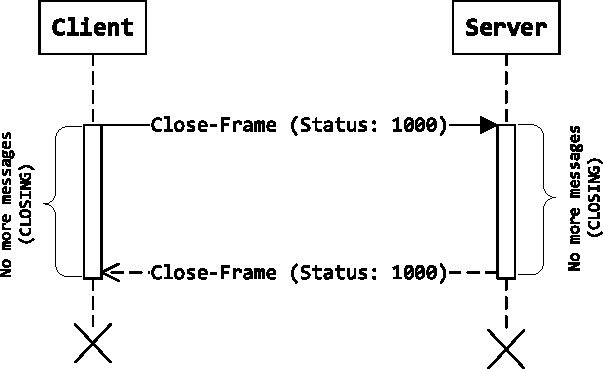
\includegraphics[scale=1]{img/closehandshake.pdf}
		\caption{Clientseitiger Closing-Handshake}
		\label{fig:wsClosingHandshake}
	\end{center}
\end{figure}

\noindent Abbildung \ref{fig:wsClosingHandshake} zeigt den schematischen Ablauf des Closing-Handshakes. Der Client initiiert diesen, indem er einen Closing-Frame mit dem Statuscode 1000 versendet. Der Server reagiert mit einer entsprechenden Antwort, wobei der Status aus dem ersten Frame übernommen wurde. Nachdem der Closing-Handshake abgeschlossen wurde befinden sich beide Endpunkte im Status \texttt{CLOSED} und die zugrundeliegende TCP-Verbindung kann beendet werden.

\subsection{Alternative Verfahren}\label{subsubsec:AlternativeVerfahren}
Die Kommunikation mittels HTTP basiert auf einem Request/Response Verfahren. Dabei sendet immer der Client eine Anfrage an einen Server. Dieser antwortet mit einer Statuszeile und entsprechendem Statuscode. Anschließend gilt die Übertragung als beendet und kann durch eine erneute Anfrage des Clients neu gestartet werden. Eine Möglichkeit Daten vom Server an den Client zu senden, ist in der Spezifikation von HTTP nicht vorgesehen. Verändert sich der Zustand einer serverseitigen Ressource, so kann der Client darüber bei einer reinen HTTP-Verbindung nur durch erneutes Anfragen informiert werden. Allerdings benötigen viele Anwendungsfälle diese Funktion. Aus diesem Grund wurde eine Vielzahl von Verfahren entwickelt, die diese Mechanismen abbilden sollen. Im Folgenden werden einige dieser Verfahren kurz vorgestellt und hinsichtlich ihrer Vor- und Nachteile gegenüber WebSocket analysiert.\\

\subsubsection{Polling}
Durch die vom W3C standardisierte API XMLHttpRequest (XHR) wurde im Jahr 2012 eine Möglichkeit geschaffen, mittels JavaScript HTTP-Requests zu konstruieren \autocite{whatwg_xmlhttprequest_2006}. Ein XHR-Objekt registriert verschiedene Methoden, welche bei einer Änderung des Objekts asynchron aufgerufen werden. Dadurch können Anfragen gesendet werden, ohne den weiteren Programmablauf zu blockieren. Dies bildet die technische Grundlage vieler moderner Web-Frontends, die unter dem Oberbegriff Ajax (\textit{Asynchronous JavaScript and XML}) zusammengefasst werden \autocite[26]{gorski_websockets_2015}. \\

\noindent Beim Polling-Verfahren wird eine Anfrage an den Server in festgelegten Zeitabständen wiederholt. Durch die Verwendung eines XHR-Objekts blockiert die Anwendung zwischen dem Absenden und Empfang der Serverantwort nicht. Liegt keine Änderung vor, so sendet der Server eine leere Antwort zurück. \\

\noindent Dieses Verfahren wird von allen Browsern unterstützt und bedarf keiner besonderen Kenntnisse. Allerdings ist der erzeugte Overhead je nach Einsatzszenario nicht zu unterschätzen. Auch die Belastung des Servers bei der Verarbeitung der eintreffenden Anfragen kann problematisch sein. Treten demnach viele Änderungen in kurzen Zeitabständen auf, so ist von der Verwendung eines einfachen Polling-Verfahrens abzuraten.

\subsubsection{Long-Polling}\label{subsubsec:Long-Polling}
Die regelmäßigen Abfragen des einfachen Pollings führen zu einem enormen Overhead. Um diesen zu reduzieren wird beim Long-Polling nur eine Antwort vom Server zurückgesendet, wenn eine Änderung vorliegt. Der Client reagiert umgehend mit einem neuen Request auf die Antwort des Servers. Die Verbindung bleibt dabei geöffnet, solange keine Änderung auftritt. Läuft die vordefinierte Wartezeit ab, so antwortet der Server auch hier mit einer leeren Nachricht \autocite[29]{gorski_websockets_2015}. \\

\noindent Das Long-Polling reduziert den Overhead gegenüber dem einfachen Polling-Mechanismus deutlich. Auf Grund des sofortigen Wiederaufbaus durch den Client wird eine nahezu andauernde Verbindung simuliert. Dennoch ist auch in diesem Fall der Overhead deutlich größer als bei der Verwendung einer WebSocket-Verbindung. Mit steigender Frequenz von Nachrichten nähert sich dieser an den Overhead des einfachen Pollings.

\subsubsection{Comet}\label{subsubsec:Comet}
Auf Grund diverser Limitierungen für Mehrbenutzeranwendungen, entwickelten sich Programmiermodelle, welche unter der Bezeichnung \textit{Comet} \autocite{russell_comet_2006} zusammengefasst wurden. Da es sich hierbei nicht um einen spezifizierten Standard handelt, wurde im Rahmen des CometD-Projekts der Dojo Foundation das Bayeux-Protokoll ins Leben gerufen. Ziel des Projekts ist die Reduzierung der Komplexität bei der Implementierung von Comet Anwendungen \autocite{russell_cometd_2007}. Um dies zu erreichen wurden Referenzimplementierungen des Bayeux-Protokolls in verschiedenen Programmiersprachen bereitgestellt. \\

\noindent Neben der Verwendung des Long-Polling Mechanismus zur ereignisgesteuerten Nachrichtenübertragung von Server zu Client, sieht das Bayeux-Protokoll auch Streaming-Techniken vor. Dabei wird die HTTP-Verbindung nach der Antwort des Servers auf den Request des Clients nicht geschlossen, sondern anhand des Connection-Headers \texttt{keep-alive} weiterhin offen gehalten. Somit können weitere Nachrichten vom Server an den Client gesendet werden, ohne dass eine erneute Anfrage durch den Client gestellt werden muss. \\

\begin{figure}[ht] 
	\begin{center}
		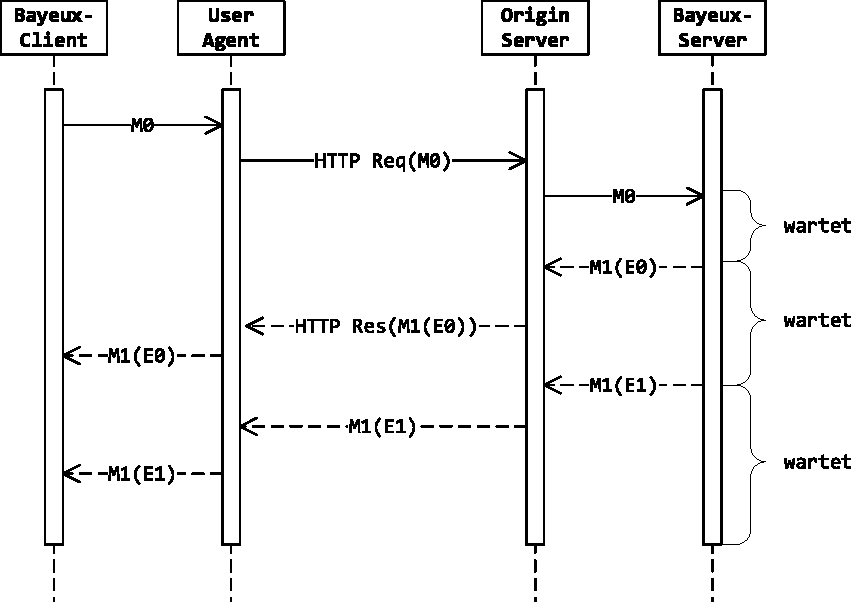
\includegraphics[scale=1]{img/bayeuxstream.pdf}
		\caption{HTTP-Streaming im Bayeux-Protokoll}
		\label{fig:wsBayeuxStream}
	\end{center}
\end{figure}

\noindent Allerdings muss die Verwendung von HTTP-Streaming von den User Agenten unterstützt werden, da unvollständige HTTP Responses für dieses Verfahren genutzt werden \autocite{russell_cometd_2007}. Um bidirektional kommunizieren zu können verwendet das Bayeux-Protokoll zwei HTTP-Verbindungen, wohingegen das WebSocket-Protokoll mit einer einzigen Verbindung arbeitet. Der größte Nachteil des Bayeux-Protokolls ist jedoch die fehlende Standardisierung durch eine etablierte Organisation. 

\subsubsection{Server-Sent Events}\label{subsubsec:Server-SentEvents}
Die bislang vorgestellten Verfahren bieten keine standardisierte API, die es Servern ermöglicht Daten über HTTP an eine Website zu senden. In HTML5 wurde dafür vom W3C die sogenannten \textit{Server-Sent Events (SSE)} eingeführt, welche ein \texttt{EventSource}-Objekt bereitstellen. Dieses sorgt auf der Clientseite dafür, dass Benachrichtigungen des Servers empfangen werden können. Dazu stellt der Browser drei Event-Handler bereit, die DOM-Events an die Anwendung weiterleiten \autocite[31]{gorski_websockets_2015}. Bei der Öffnung einer SSE-Verbindung wird der Event-Handler \texttt{onopen} aufgerufen, im Falle eines Fehlers der \texttt{onerror}-Handler. Kommen Nachrichten des Servers an, so wird der \texttt{onmessage}-Handler aktiviert \autocite{hickson_server-sent_2009}. Zu jedem Event-Handler werden entsprechende Methoden registriert, welche die Bearbeitung des jeweiligen Events übernehmen.\\

\noindent Server-Sent Events erzeugen keinen Overhead durch wiederholte Anfragen an den Server. Die Kommunikation von Server zu Client wird ermöglicht, ohne mehrere HTTP-Verbindungen zu öffnen. Allerdings handelt es sich hier um einen unidirektionalen Kanal von Server zu Client. Dies ist für Anwendungsfälle ausreichend, in denen lediglich der Server Informationen zu übermitteln hat. Beispiele hierfür wären u.a. das Hardware-Monitoring eines Server oder ein Newsticker. Sollen jedoch Daten in beide Richtungen übertragen werden, so ist die Verwendung von WebSockets die bessere Alternative. Insbesondere Mehrbenutzeranwendungen wie Spiele oder Chats, die auf kurze Latenzen angewiesen sind, profitieren von derem bidirektionalem Kommunikationskanal.

\section{Die WebSocket API}\label{sec:WebSocketAPI}
\subsection{Client-seitige Implementierung}
\subsection{Server-seitige Implementierung}

\section{Fachliche Anforderungen}
\subsection{Analyse des DaKo-Frameworks}
\subsection{Anforderungen an WebSocket-Chat}
\subsection{Prototypische Implementierung}

\section{Technische Anforderungen}
\subsection{Entwurf des WebSocket-Chats}
\subsection{Vergleich der Implementierungsformen}
\subsection{Implementierung des WebSocket-Chats}

\section{Evaluation}
\subsection{Test-Umgebung}
\subsection{Leistungsanalyse WebSocket-Chat}

\section{Zusammenfassung und Ausblick}
\subsection{Einsatzgebiete}
% Unterschrift (handgeschrieben)

\newpage
\pagenumbering{Roman}
\printbibliography
\newpage
\listoffigures
\newpage
\listoftables

\end{document}
